\newpage
\section{Auswertung}
    \subsection{Statische Methode}
        Bei der statischen Methode wird jeweils an zwei Stellen eines jeden Metallstabes die Temperatur als Funktion der Zeit gemessen und über den zeitlichen
        Temperaturverlauf wird an den beiden Messstellen die Wärmeleitfähigkeit der vier Metallstäbe bestimmt.

        \subsubsection{Temperaturverläufe der fernen Thermoelemente}
        Im folgenden befindet sich eine Grafik für die fernen Thermoelemente. Dabei misst das Thermoelement $T_1 \si{second}$ an dem dicken Messingstück und $T_4 \si{second}$ am dünnen. $T_5 \si{second}$ und $T_8 \si{second}$ sind
        jeweils am Aluminium und Edelstahl befestigt.

        \begin{figure}
               \centering
               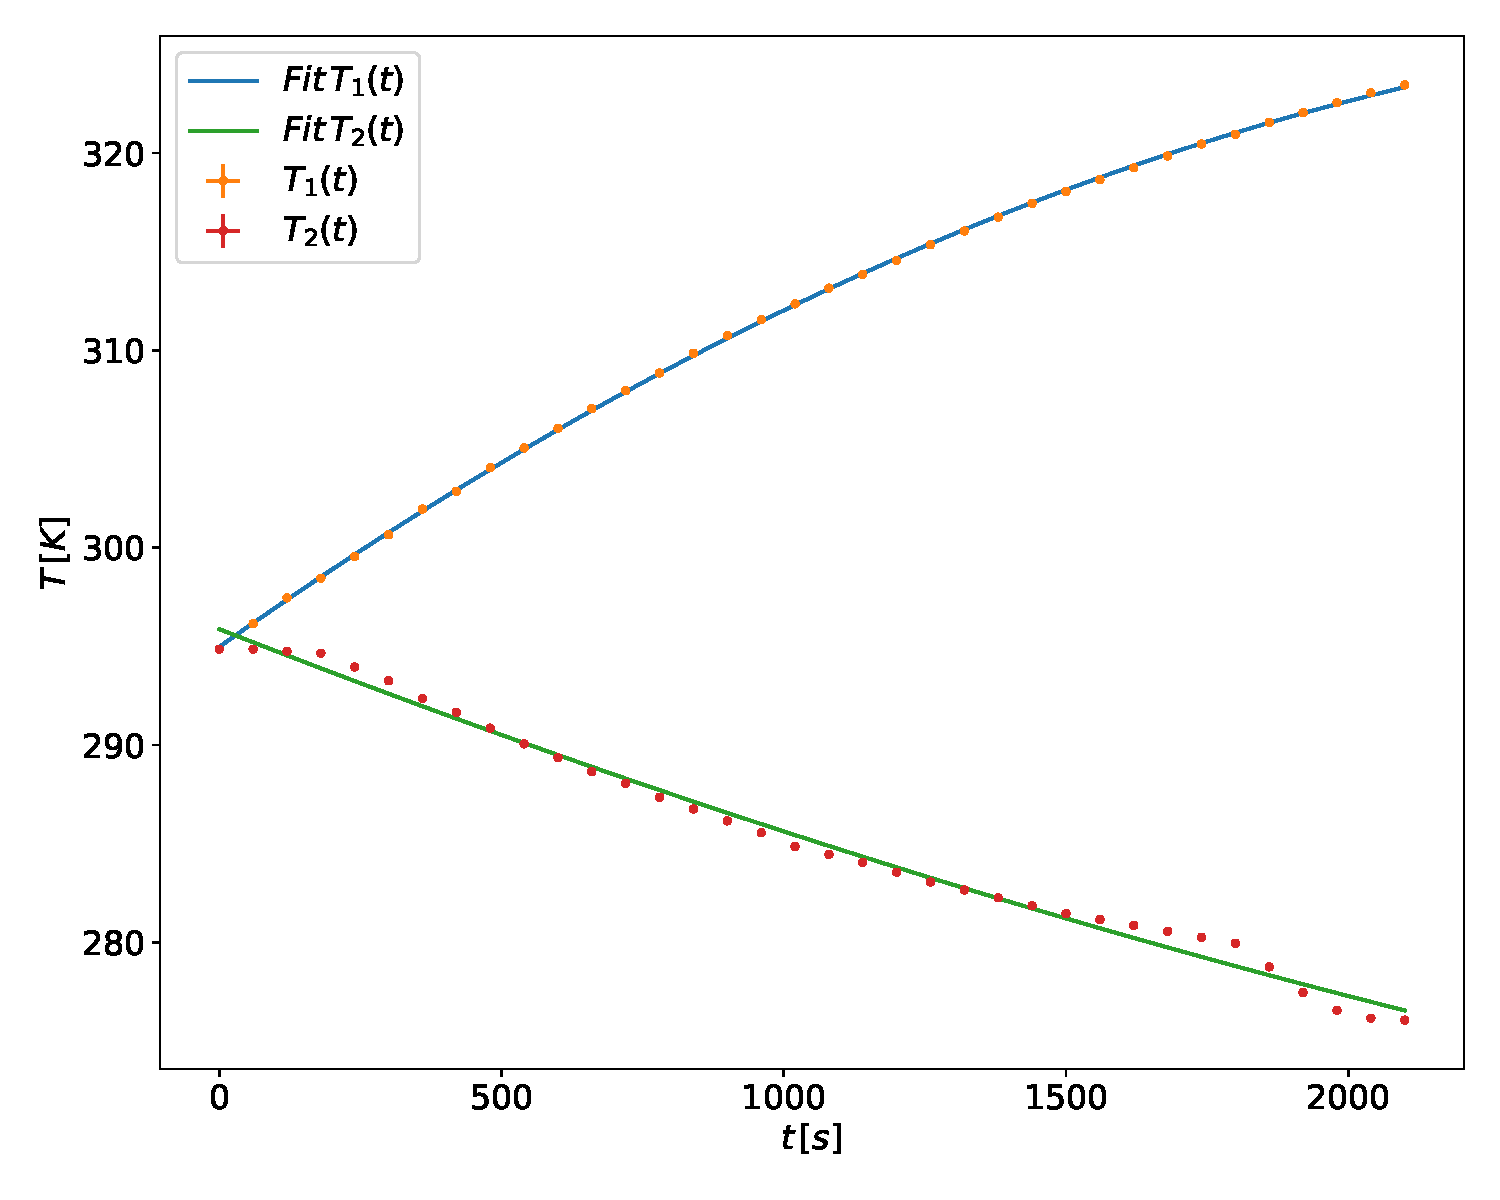
\includegraphics[width=\textwidth]{Daten/grafic.pdf}
               \caption{Temperaturverläufe der fernen Thermoelemente $T_1$, $T_4$, $T_5$, $T_8$}
               \label{fig:static_far}
        \end{figure}

        Es fällt auf, dass $T_1$ und $T_4$ ungefähr von $t = 0 \si{second}$ bis $t = 100 \si{second}$ gleichstark steigen, jedoch steigt die Temperatur von $T_5$ deutlich steiler und von $T_8$ deutlich 
        flacher als die gemessene Temperatur der anderen Thermoelemente.
        Zudem ist bei allen Thermoelementen, außer bei $T_8$, ab $t = 600 \si{second}$ ein starker Knick zu beobachten.




